%!TEX root = /Users/stevenmartell/Documents/iSCAM-project/docs/iSCAM-guide/userGuide/usrGuide.tex
The concept of maximum sustainable yield, or MSY, is based on the notion that the underlying stock-size versus productivity can be estimated with some degree of certainty, and that this production function is stationary over time.  For a single fishing fleet, this can easily be represented as the equilibrium catch versus the equilibrium fishing effort (Fig. \ref{fig:iscamFigs_Fig1Quadplot}a), hereafter referred to as a yield curve. In the case of multiple fishing fleets, this yield curve  is not necessarily a smooth function as the total yield summed over all fleets is also a function of the fishing mortality exerted by each of the fleets.  In section \ref{ssub:msy_based_reference_points} a description of the equilibrium yields and MSY-based reference points is given, followed by a description of the numerical methods used to obtain MSY-based reference points when there are two or more fleets fishing simultaneously.

A special class library to implement the MSY-based reference point calculations was developed specifically for \iscam.  The C++ code for this class can be found in \texttt{msy.cpp}.


\subsubsection{MSY based reference points: single fleet} % (fold)
\label{ssub:msy_based_reference_points}



In the case of a single fishery \iscam\ calculates \fmsy\ based reference points by finding the value of $F_e$ that results in the zero derivative of \eqref{T2.14}.  This is accomplished numerically using a Newton-Raphson method where an initial guess for \fmsy\ is set equal to 1.0$M$, then use \eqref{eq1.1} to iteratively find \fmsy.  Note that the partial derivatives in \eqref{eq1.1} can be found in Table~\ref{tab:partial_derivatives}.

\begin{align}\label{eq1.1}
    F_{e+1}&=F_e - 
    \dfrac{ \dfrac{\partial C_e}{\partial F_e}}
    { \dfrac{\partial C_e^2}{\partial F_e^2}}\\
    \mbox{where}\nonumber\\
     \frac{\partial C_e}{\partial F_e} &=
    R_e \phi_q
    + F_e \phi_q \dfrac{\partial R_e}{\partial F_e}
    + F_e R_e \dfrac{\partial \phi_q}{\partial F_e} \nonumber\\
    \frac{\partial C_e^2}{\partial F_e^2} &=
    \phi_q \dfrac{\partial R_e}{\partial F_e}
   +  R_e \dfrac{\partial \phi_q}{\partial F_e}\nonumber
%    \frac{R_e \phi_q
%    + F_e \phi_q \dfrac{\partial R_e}{\partial F_e}
%    + F_e R_e \dfrac{\partial \phi_q}{\partial F_e}}
%    {\phi_q \dfrac{\partial R_e}{\partial F_e}
%    +  R_e \dfrac{\partial \phi_q}{\partial F_e}}.
\end{align}

The algorithm usually converges in less than 10 iterations depending on how close the initial guess of \fmsy\ is to the true value.  A maximum of 200 iterations are allowed in \iscam\ and if $\frac{\partial C_e}{\partial F_e}<1e-12$ it is assumed to be sufficiently close to zero and iterations will stop.  Note also, that this class object is only performed on data type variables and not differentiable variables within AD Model Builder.
 

\begin{figurehere}
    \centering
        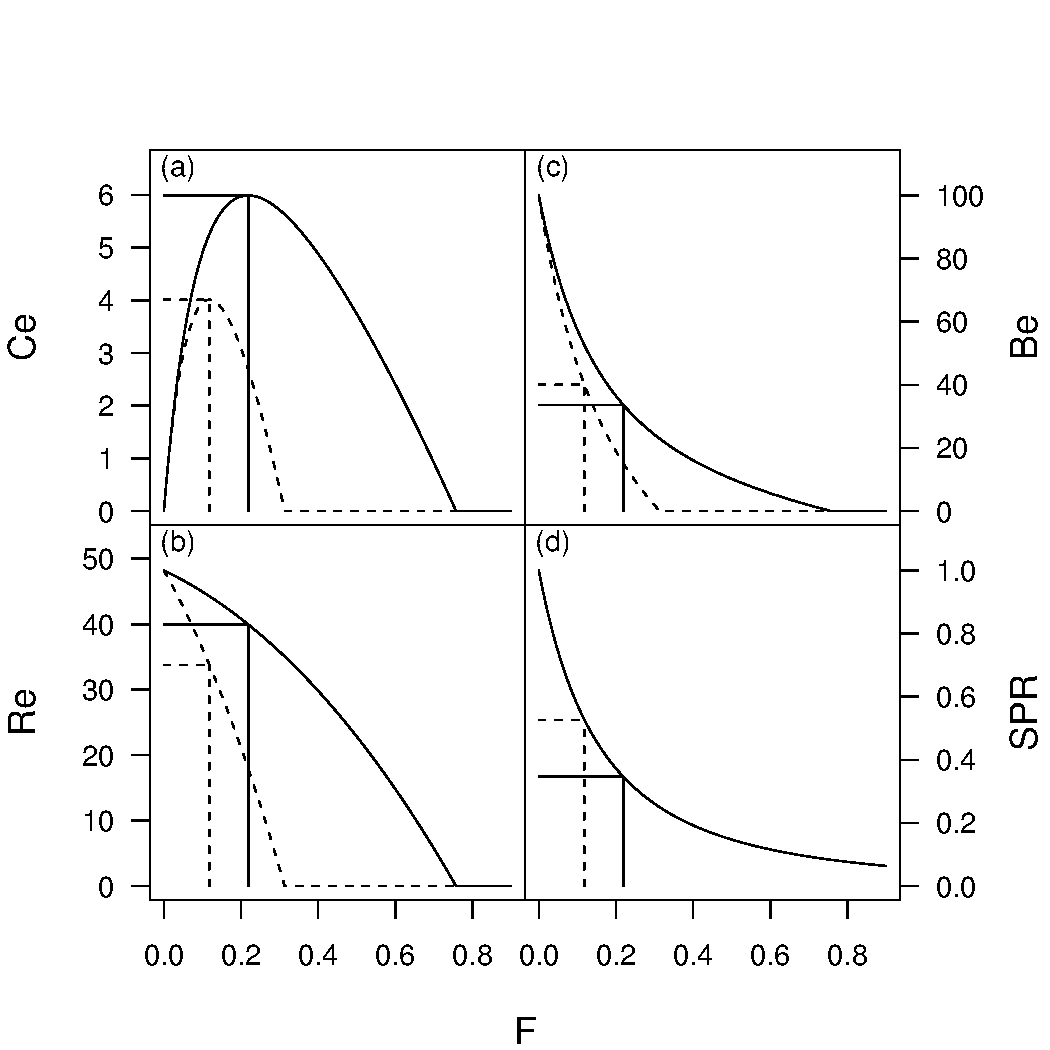
\includegraphics[height=3in]{iscamFigs/Fig1Quadplot.pdf}
    \caption{Equilibrium yield (a), recruits (b), biomass (c) and
       spawner per recruit ($\phi_e/\phi_E$) (d) versus instantaneous
       fishing mortality $F_e$ for two different values of the recruitment
       compensation ratio ($\kappa=12$ solid lines, $\kappa=4$ dashed
       lines). Vertical lines in each panel correspond to \fmsy\ and
       horizontal lines correspond to various reference points that would
       achieve MSY.}
    \label{fig:iscamFigs_Fig1Quadplot}
\end{figurehere}

Given an estimate of \fmsy, other reference points such as MSY are calculated use the equations in Table-\ref{tab:equilibrium_model} where each of the expressions is evaluated at \fmsy.  A graphical representation of MSY based reference points for two alternative values of the recruitment compensation parameter $\kappa$ is show in Figure \ref{fig:iscamFigs_Fig1Quadplot}. All other parameters in the vectors $\Theta$ and $\Phi$ are identical between the two scenarios.  A lower recruitment compensation ratio (or a lower steepness value in the stock recruitment relationship) implies lower stock productivity or less resilience to fishing. Recruitment and biomass decrease at a much faster rate with increased fishing mortality in comparison to a stock with a higher recruitment compensation ratio. Note that the spawning potential ratio (SPR) curve is insensitive to the estimated value of recruitment compensation (steepness);  however, the SPR value at which MSY is achieved increases with lower recruitment compensation (Fig \ref{fig:iscamFigs_Fig1Quadplot}d).


%%%%%%%%%%%%%%%%%%%%%%%%%%%%%%%%%%%%%%%%%%%%%%%%%%%%%%%%%%%%%%%%%%%%%%
%%%%%%%%%%%%%%%%%%%%%%%%%%%%%%%%%%%%%%%%%%%%%%%%%%%%%%%%%%%%%%%%%%%%%%
\begin{tablehere}
  \centering
\caption{Partial derivatives, based on components in Table
\ref{tab:equilibrium_model}, required for the numerical calculation of \fmsy\ using \eqref{eq1.1}.}\label{tab:partial_derivatives} \tableEq
    \begin{gather}
        \hline
        \mbox{Mortality \& Survival} \nonumber \\
        Z_{a}=M_a+F_ev_a                                \label{T3.1} \\
        S_{a}=1-e^{-Z_a}                                \label{T3.2}\\[1ex]
        %%
        %%
        \mbox{Partial for survivorship} \nonumber \\
        \frac{\partial \hat{\iota}_a}{\partial F_e} =
        \begin{cases}
          0,& a=1                                       \label{T3.3}\\
          e^{-Z_{a-1}}\left(\dfrac{\partial \hat{\iota}_{a-1}}{\partial F_e}
           -\hat{\iota}_{a-1}v_{a-1}\right),& 1<a<A\\
           \dfrac{\dfrac{\partial \hat{\iota}_{a-1}}{\partial F_e}}
           {1-e^{-Z_a}} -
           \dfrac{\hat{\iota}_{a-1} e^{-Z_{a-1}} v_a e^{-Z_a}}
           {(1-e^{-Z_a})^2}, &a=A
        \end{cases} \\[1ex]
%%        \frac{\partial \hat{\iota}_a}{\partial F_e} =
%%        \begin{cases}
%%          0,& a=1 \label{T3.3}\\
%%          e^{-Z_{a-1}}\left(\dfrac{\partial \hat{\iota}_{a-1}}{\partial F_e}
%%           -\hat{\iota}_{a-1}v_{a-1}\right),& a>1
%%        \end{cases} \\[1ex]
        %%
        %%
        \mbox{Partials for incidence functions} \nonumber \\
        \frac{\partial \phi_e}{\partial F_e}=
            \sum_{a=1}^\infty f_a \frac{\partial \hat{\iota}_a}{\partial
            F_e}                                        \label{T3.4}\\
        %%
        %%
        \frac{\partial \phi_q}{\partial F_e}=
            \sum_{a=1}^\infty \frac{w_av_a S_a}{Z_a}
             \frac{\partial \hat{\iota}_a}{\partial F_e}
             +\frac{\hat{\iota}_a w_av_a^2}{Z_a}\left(e^{-Z_a}-\frac{S_a}{Z_a} \right)
                                                            \label{T3.5}\\[1ex]
        %%
        %%
        \mbox{Partial for recruitment} \nonumber\\
        \frac{\partial R_e}{\partial F_e}=\frac{R_o}{\kappa-1}
        \frac{\phi_E}{\phi_e^2} \frac{\partial \phi_e}{\partial
        F_e}                                                \label{T3.6}\\[1ex]
        \hline \hline \nonumber
    \end{gather}

    \normalEq
\end{tablehere}
%%%%%%%%%%%%%%%%%%%%%%%%%%%%%%%%%%%%%%%%%%%%%%%%%%%%%%%%%%%%%%%%%%%%%%
%%%%%%%%%%%%%%%%%%%%%%%%%%%%%%%%%%%%%%%%%%%%%%%%%%%%%%%%%%%%%%%%%%%%%%

% subsubsection msy_based_reference_points (end)

\subsubsection{MSY Based Reference Points: two or more fleets} % (fold)
\label{ssub:msy_based_reference_points_two_or_more_fleets}

In the case where there are two or more fishing fleets with distinctly different selectivity curves for each of the fleets, determination \fmsy for each of the fleets is a bit more complicated.  The first major complication is solving the catch equation where \eqref{T2.14} now involves a summation term over different fishing fleets.  The second complication is how should the total catch (summed over fleets) be allocated to each of the fleets.  In the special case where selectivity for each of the fishing fleets is identical, an equal proportion of the total catch allocated to each of those fleets also corresponds to the same fishing mortality for each of those fleets.  In the more common case where selectivity differs among fleets, the fishing mortality rates associated with equal allocations would also differ.  Consider the following example, if you have a purse seine fleet that harvests small young tuna, and a long-line fleet that harvest the same stock but selects larger older tuna. If each of these two fleets are allocated a 50:50 share, the instantaneous fishing mortality rate would have to be much higher for the long-line gear relative to the purse seine gear that harvest the more abundance small/young tuna.  Regarding the first complication, the following description is based on the assumption is that the total catch summed over all fleets is maximized, and that allocation of total catch is a secondary issue. For the second complication, a vector of fishing mortality rate multipliers is used to adjust fleet specific fishing mortality rates to satisfy catch allocations.  Lastly, a third complication pertains to the accounting of mature numbers-at-age at the time of spawning and how much of the total annual mortality occurs prior to spawning. 


% From msy.cpp
The steady-state catch equation for fleet $k$, with an instantaneous fishing mortality rate $F_k$, is given by:
\begin{align}
	C_{k} &= F_k R_e \phi_{q,k} \label{eq:C_k}\\
	\mbox{where}\nonumber\\
	R_e &= \frac{R_o (\kappa-\phi_E/\phi_e)}{\kappa-1} \label{eq:R_e}\\  %ro*(kappa-m_phie/phif) / km1;
	\phi_{q,k} &= \sum_j = \frac{e^{-M(j-1)}V_{k,j}w_a (1-e^{-M-\sum_k F_k V_{k,j} })}{M+\sum_k F_k V_{k,j}} \label{eq:phi_qk}
\end{align}

Although the catch equation appears relatively simple, there are two key points to note about the equilibrium recruitment $R_e$ and the yield per recruit $\phi_{q,k}$ in \eqref{eq:R_e} and \eqref{eq:phi_qk}, respectively. First, \eqref{eq:R_e} is a function of the eggs per recruit under fished conditions $\phi_e$, which is based on the survivorship which depends on the fishing mortality rates of all gears.  Second, the yield per recruit in \eqref{eq:phi_qk} is a function of the total mortality rate which involves the summation over gears.

The maximum total yield summed over all $k$ fleets occurs under the following condition:
\begin{equation}
	0 = \sum_k \frac{\partial C_k}{\partial F_k}  \label{eq:Catch_derivative}
\end{equation}
and thus the goal is to find a vector of steady-state fishing mortality rates $F_k$ to satisfy \eqref{eq:Catch_derivative}.  


% subsubsection msy_based_reference_points_two_or_more_fleets (end)


\subsubsection{Reference points for multiple fisheries with fixed allocation} % (fold)
\label{ssub:reference_points_for_multiple_fisheries}
% It is common that a single stock of fish is prosecuted by many different types of fishing gears that have differing selectivities.  In such cases, the definition of MSY is based on the sum of catches from each of the participating fleets and how much of the total catch is taken, or allocated, to specific sectors.  For such cases, it is still possible to calculate MSY-based reference points provided that allocation to each of the gear types is specified \emph{a priori}.

To determine MSY-based reference points for 2 or more gear types (e.g.,  purse seine and gillnet fisheries for Pacific herring in British Columbia), \iscam\ requires an allocation for each of the defined fleets.  Allocation is specified in the data file (see sub section \ref{sub:the_data_file}).  This allocation is initially used set a series of F-multipliers ($\lambda_k$) for each gear and \eqref{T2.14} becomes a vector of catches:
\begin{align}
	C_{e,k} &= F_e \lambda_k R_e \phi_{q,k} \label{eq:12} \\
	&\mbox{where the per-recruit yield for gear $k$ is:} \nonumber \\
	Z_a &= M+F_e\sum_k \lambda_kv_{k,a}\label{eq:13}\\
	\phi_{q,k}&=\sum_{a=1}^\infty
        \frac{ \hat{\iota}_a \lambda_k w_a v_{k,a}}{Z_a}
        \left(1-e^{Z_a}\right)\label{eq:14}\\
    &\mbox{with the added constraint} \nonumber\\
    \sum_k \lambda_k &= N \label{eq:15}\quad \mbox{where $N$ is the number of gears.}
\end{align}

The constraint in \eqref{eq:15} defines $F_e\lambda_k$ as the fishing mortality rate for gear $k$ where $\lambda_k$ is a multiple of the average fishing mortality rate of all gears.  To ensure that each gear achieves the specified allocation for a given average fishing mortality rate $F_e$, the multipliers are determined iteratively where $\lambda_k$ is updated using:
\begin{align}
	\lambda_k^{(i+1)} &= \lambda_k^{(i)} \frac{a_k}{p_k} \label{eq:16}\\
	&\mbox{where $a_k$ is the allocation for gear $k$, and:}\nonumber\\
	p_k &= \frac{C_{e,k}}{\sum_k C_{e,k}}\label{eq:17}
\end{align}
Depending on the differences in selectivities and allocations between the gear types, this algorithm converges roughly 7-15 iterations.  From here the same Newton-Raphson algorithm is used to determine the average fishing mortality rate $F_e$ that would maximize the sum of catches over the multiple gears.  
% subsubsection reference_points_for_multiple_fisheries (end)



\subsection{MSY-based reference points for multiple fisheries} % (fold)
\label{sub:msy_based_reference_points_for_multiple_fisheries}

In cases where there are two or more fishing fleets that harvest the same stock (intentionally or taken as bycatch), the differences in selectivity among these gears will ultimately affect the fishing mortality rates associated with long-term sustainable yields or MSY for each of the participating fleets.  For example, global tuna fisheries are taken primarily by two gear types, pelagic longlines which harvest larger/older tuna, and purse seine's which harvest younger tuna usually aggregated around Fish Aggregating Devices (FADs).  The longline fishery has been in operation since the 1950s (even longer, but the available data date back to the 1950s), and the industrial purse seine fishery developed in the 1980s.  If in fact the longline fishery was fully utilized by the 1980s, then the impacts of increased mortality on younger tuna from the purse seine fleet would reduce the available surplus for the longline fishery.

To estimate what the appropriate MSY-based fishing mortality rates for two or more fishing gears that harvest the same stock of fish, the catch equations for each fleet must be simultaneously solved in order to find the appropriate vector of fishing mortality rates that that maximizes the yields for each fleet.  The steady-state, or equilibrium, catch equation for a given fishing gear $k$ is given by:
\begin{equation}\label{eq:equilYield}
	 Y_{k} = \sum_j\frac{N_j F_k v_{k,j} w_j (1-\exp(-M-\sum_k F_k v_{k,j}))} {M + \sum_k F_k v_{k,j}},
\end{equation}
where $F_k$ is the fishing mortality rate imposed by gear $k$, M is the instantaneous natural mortality rate, $v_{k,j}$ is the age-specific selectivity for gear $k$ and age$j$, and $w_j$ and $N_j$ are the average weight-at-age and numbers-at-age, respectively.  Note that if $k>1$, then \eqref{eq:equilYield} represents of system of nonlinear equations where the roots of these equations $\left(\frac{\partial Y_k}{\partial F_k}=0\right)$ are found with Newton-Raphson.

\subsubsection{Algorithm for estimating \fmsy\ for multiple fleets} % (fold)
\label{ssub:algorithm_for_estimating_fmsy_for_multiple_fleets}


% subsubsection algorithm_for_estimating_fmsy_for_multiple_fleets (end)

% subsection msy_based_reference_points_for_multiple_fisheries (end)

